\subsection{Julia}
Julia è un linguaggio di programmazione ad alto livello, 
multi-paradigma e open-source ideato per compiere analisi 
numerica ed effettuare operazioni di computer science in 
maniera rapida e stabile. Julia è nato ufficialmente come 
linguaggio di programmazione nell’anno 2012 con lo scopo di 
fornire uno strumento potente, robusto e veloce tanto se non 
più dei linguaggi considerati in questo ambito lo stato 
dell’arte, ovvero C e Fortran;  ma anche facile da approcciare, 
al contrario dei linguaggi sopra citati. Julia è un linguaggio 
di programmazione scritto in C++ e Scheme, ma gran parte della 
sua composizione è scritta in Julia stesso 
\cite{wiki:Julia_(programming_language)}.

\begin{figure}
    
\includegraphics[width=\linewidth]{img/Julia_Programming_Language_Logo.svg.png}
    \caption{Logo del linguaggio di programmazione Julia}
    \label{fig:Julia_logo}
\end{figure}

le caratteristiche principali di questo linguaggio sono 
principalmente:
\begin{itemize}
    \item Alte performance: lo scopo per cui Julia è nato è 
    stato quello di offrire un linguaggio estremamente 
    performante con la capacità di poter compilare programmi 
    in codice nativo per molteplici piattaforme grazie 
    all’utilizzo di LLVM

    \begin{figure}
        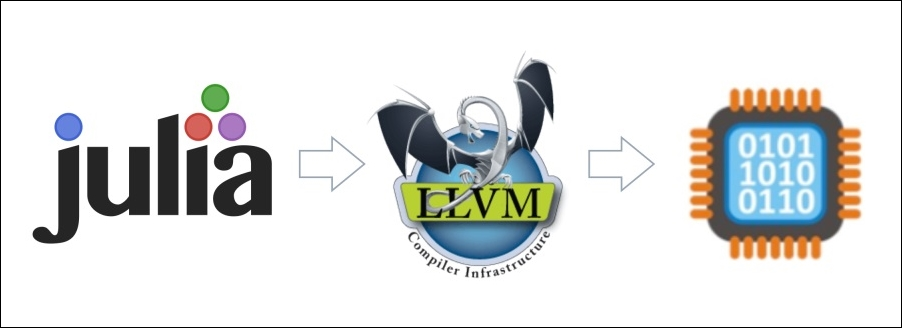
\includegraphics[width=\linewidth]{img/julia_llvm.jpg}
        \caption{Esempio struttura Julia e LLVM}
        \label{fig:Julia_LLVM}
    \end{figure}

    \item Dinamico: la scelta di rendere Julia un linguaggio 
    dinamicamente tipizzato lo rende di facile utilizzo in 
    quanto rende molto più semplice il suo approccio anche a 
    chi non ha una base solida di programmazione, in quanto 
    ritorna la stessa sensazione di immediatezza di un 
    linguaggio di scripting. Inoltre questo permette un alto 
    supporto per l’uso interattivo

    \begin{figure}
        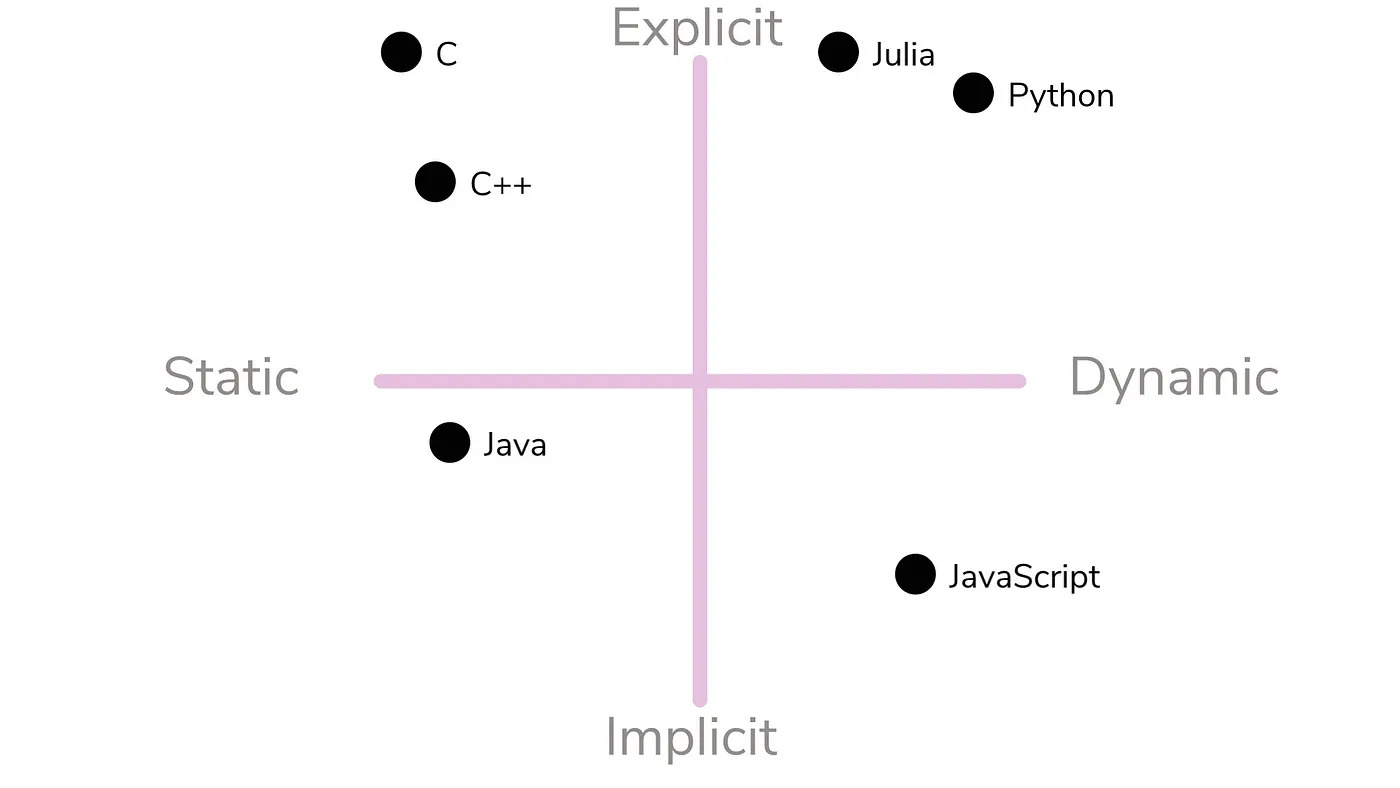
\includegraphics[width=\linewidth]{img/typing_example.jpg}
        \caption{Esempio differenze di typing in alcuni linguaggi di programamzione}
        \label{fig:Different_typing}
    \end{figure}

    \item Ambiente riproducibile: lo scopo del linguaggio è 
    quello di poter permettere all’utente di ricreare le 
    stesse condizioni ogni volta su ogni macchina su cui un 
    programma viene eseguito. Questo può essere ottenuto 
    tramite l’utilizzo di file binari pre compilati
    \item Componibile: Julia utilizza l’approccio multiple 
    dispatch come paradigma, permettendo una grande 
    flessibilità nell’esprimere una elevata quantità di 
    pattern di programmazione, dall’object-oriented al 
    funzionale
    \item General Purpouse: lo scopo del linguaggio è quello 
    di creare un ecosistema in grado di poter soddisfare 
    qualsiasi esigenza di un utente, permettendo la creazione 
    di applicativi e microservizi senza dover ricorrere ad 
    integrazioni con codice non nativo Julia
    \item Open source: Julia abbraccia la filosofia open source, 
    e il codice sorgente dell’intero linguaggio, così come di 
    tutte le librerie è disponibile sulla piattaforma GitHub 
    sotto la licenza MIT. Questo permette una crescita 
    eterogenea grazie al contributo di più di 1000 utenti 
    che si impegnano a migliorare il linguaggio
\end{itemize}

\subsubsection{Agents.jl}
Seguendo la filosofia propria del linguaggio di programmazione 
in cui è sviluppata, la libreria Agents.jl \cite{Agents.jl} 
viene sviluppata con l’obiettivo di essere facile da imparare e 
usare ed estendibile, con forte attenzione sulla creazione ed 
evoluzione di modelli veloci e soprattutto scalabili. 
Molteplici esempi comparativi sono stati effettuati mostrando 
come il framework sviluppato permetta di avere un notevole 
guadagno prestazionale rispetto ai maggiori competitor 
attualmente presenti sul mercato (Mesa, Netlogo, MASON) 
\cite{ABAR201713}.

La facilità di interazione con questa libreria non è da 
confondersi con una mancanza di opzioni durante lo sviluppo, 
in quanto nativamente Agents.jl permette l’integrazione con 
altre librerie che in maniera altrettanto semplice e veloce 
offrono all’utente la possibilità 
di addentrarsi nel mondo del machine learning, in particolar 
modo il mondo del Scientific Machine Learning 
\cite{rackauckas2017differentialequations}, 
branca che soprattutto grazie alla pandemia da Covid-19 ha 
visto un enorme interesse per l’analisi di dati per lo 
sviluppo di policy di prevenzione e contenimento della 
pandemia. 

\begin{figure}
    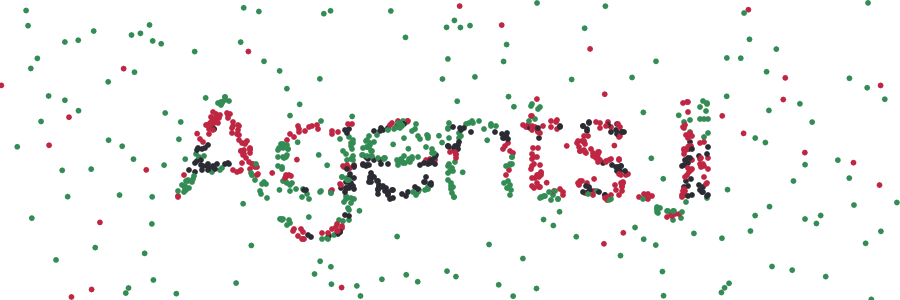
\includegraphics[width=\linewidth]{img/Agents_5poOwRo.png}
    \caption{Logo framework Agents.jl}
    \label{fig:Agents.jl_logo}
\end{figure}

\subsubsection{SciML.ai}
SciML è una collezione di librerie dedite al calcolo scientifico 
e non solo al machine learning. Questo framework permette di 
avere tutti gli strumenti per poter utilizzare facilmente, 
velocemente e in maniera robusta tecniche di analisi numerica 
molto avanzata, così da poter sviluppare applicazioni 
semplicemente senza essere banali 
\cite{rackauckas2017differentialequations} 
\cite{rackauckas2019diffeqflux} 
\cite{rackauckas2020universal}. 

\begin{figure}
    
\includegraphics[width=\linewidth]{img/SciMLGitHubPreview.png}
    \caption{Logo SciML.ai}
    \label{fig:SciML.ai}
\end{figure}

Durante la pandemia da Covid-19 questo framework è stato 
utilizzato per sviluppare applicazioni le quali grazie 
all’utilizzo di tecniche di scientific machine learning 
riuscivano sia a prevedere in maniera molto accurata 
l’andamento dell’epidemia seppur in presenza di una scarsa 
quantità di dati (uno dei grandi problemi dei modelli di 
machine learning e di artificial intelligence sono gli enormi 
dataset necessari per addestrare le reti in maniera robusta) 
e le stesse presentavano misure di contenimento e prevenzione 
che si sono dimostrate essere efficaci 
\cite{10.1371/journal.pdig.0000142} \cite{DANDEKAR2021100220}. 

\subsubsection{SafeBlues}
Un esempio di un modello di scientific machine learning può 
essere il modello denominato SafeBlues 
\cite{10.1371/journal.pdig.0000142} \cite{DANDEKAR2021100220} il quale simulando una 
rete bluetooth in cui gli individui potevano venire infettati 
da un virus e poi infettare a loro volta tutti gli individui 
nella rete con una certa probabilità, aveva riprodotto 
fedelmente l’andamento della pandemia da Covid-19. 
In aggiunta questa soluzione, aveva mostrato come 
l’applicazione di policy per il contenimento del virus 
bluetooth erano perfettamente applicabili anche al caso 
reale della pandemia. 

\begin{figure}
    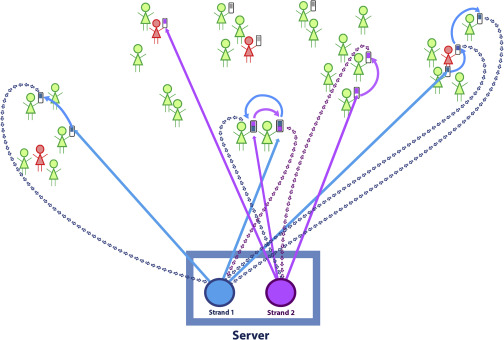
\includegraphics[width=\linewidth]{img/gr2.jpg}
    \caption{Esempio funzionamento SafeBlues}
    \label{fig:SafeBlues_1}
\end{figure}

\begin{figure}
    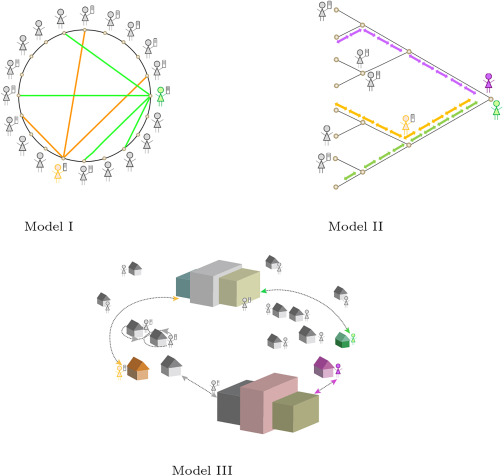
\includegraphics[width=\linewidth]{img/gr3.jpg}
    \caption{Esempio modelli SafeBlues}
    \label{fig:SafeBlues_models}
\end{figure}